\documentclass[12pt]{article}
\usepackage{graphicx,import}
\usepackage[svgnames]{xcolor} 
\usepackage{fancyhdr}
\usepackage{subfig}
\usepackage{hyperref}
\usepackage{enumitem}
\usepackage[many]{tcolorbox}
\usepackage{listings}
\usepackage{physics}
\usepackage{amsmath}
\usepackage{tikz}
\usepackage{mathdots}
\usepackage{yhmath}
\usepackage{cancel}
\usepackage{color}
\usepackage{siunitx}
\usepackage{array}
\usepackage{multirow}
\usepackage{amssymb}
\usepackage{gensymb}
\usepackage{tabularx}
\usepackage{extarrows}
\usepackage{booktabs}
\usetikzlibrary{fadings}
\usetikzlibrary{patterns}
\usetikzlibrary{shadows.blur}
\usetikzlibrary{shapes}

\usepackage[a4paper, total={6in, 8in} , bottom = 25mm , top = 25mm, headheight = 1.25cm , includehead,includefoot,heightrounded ]{geometry}
\usepackage{afterpage}
\usepackage{amssymb}
\usepackage{pdflscape}
\usepackage{gensymb}
\usepackage{textcomp}
\usepackage{tikz,pgfplots}
\usepackage{xecolor}
\usepackage{rotating}
\usepackage{pdfpages}
\usepackage[T1]{fontenc}
\usepackage{tikz}
\usepackage[utf8]{inputenc}
\usepackage{PTSerif} 
\usepackage{seqsplit}
\usepackage{fancyvrb}
\usepackage{mips}
\usepackage{multirow}
\usepackage{hhline}
\usepackage[edges]{forest}
\usepackage{tabularx}
\usepackage{float}
\usepackage{graphicx}
\usepackage{cprotect}
\usepackage{url}
\usepackage{listings}
\usepackage{xcolor}
\usepackage{pifont}
\newcommand{\xmark}{\ding{55}}%
\def\checkmark{\tikz\fill[scale=0.4](0,.35) -- (.25,0) -- (1,.7) -- (.25,.15) -- cycle;}

\hypersetup{
	colorlinks   = true, %Colours links instead of ugly boxes
	urlcolor     = blue, %Colour for external hyperlinks
	linkcolor    = blue, %Colour of internal links
	citecolor   = red %Colour of citations
}

\definecolor{codegreen}{rgb}{0,0.6,0}
\definecolor{codegray}{rgb}{0.5,0.5,0.5}
\definecolor{codepurple}{rgb}{0.58,0,0.82}
\definecolor{backcolour}{rgb}{0.95,0.95,0.92}
\definecolor{mGreen}{rgb}{0,0.6,0}
\definecolor{mGray}{rgb}{0.5,0.5,0.5}
\definecolor{mPurple}{rgb}{0.58,0,0.82}
\definecolor{backgroundColour}{rgb}{0.95,0.95,0.92}

\NewDocumentCommand{\codeword}{v}{
	\texttt{\textcolor{blue}{#1}}
}
\lstset{language=java,keywordstyle={\bfseries \color{blue}}}
\definecolor{dkgreen}{rgb}{0,0.6,0}
\definecolor{gray}{rgb}{0.5,0.5,0.5}
\definecolor{mauve}{rgb}{0.58,0,0.82}



\lstdefinestyle{mystyle}{
	backgroundcolor=\color{backcolour},   
	commentstyle=\color{codegreen},
	keywordstyle=\color{magenta},
	numberstyle=\tiny\color{codegray},
	stringstyle=\color{codepurple},
	basicstyle=\ttfamily\normalsize,
	breakatwhitespace=false,         
	breaklines=true,                 
	captionpos=b,                    
	keepspaces=true,                 
	numbers=left,                    
	numbersep=5pt,                  
	showspaces=false,                
	showstringspaces=false,
	showtabs=false,                  
	tabsize=2
}

\lstdefinestyle{CStyle}{
	backgroundcolor=\color{backgroundColour},   
	commentstyle=\color{mGreen},
	keywordstyle=\color{magenta},
	numberstyle=\tiny\color{mGray},
	stringstyle=\color{mPurple},
	basicstyle=\footnotesize,
	breakatwhitespace=false,         
	breaklines=true,                 
	captionpos=b,                    
	keepspaces=true,                 
	numbers=left,                    
	numbersep=5pt,                  
	showspaces=false,                
	showstringspaces=false,
	showtabs=false,                  
	tabsize=2,
	language=C
}



\lstset{ %
	language=[mips]Assembler,       % the language of the code
	basicstyle=\footnotesize,       % the size of the fonts that are used for the code
	numbers=left,                   % where to put the line-numbers
	numberstyle=\tiny\color{gray},  % the style that is used for the line-numbers
	stepnumber=1,                   % the step between two line-numbers. If it's 1, each line
	% will be numbered
	numbersep=5pt,                  % how far the line-numbers are from the code
	backgroundcolor=\color{white},  % choose the background color. You must add \usepackage{color}
	showspaces=false,               % show spaces adding particular underscores
	showstringspaces=false,         % underline spaces within strings
	showtabs=false,                 % show tabs within strings adding particular underscores
	frame=single,                   % adds a frame around the code
	rulecolor=\color{black},        % if not set, the frame-color may be changed on line-breaks within not-black text (e.g. commens (green here))
	tabsize=4,                      % sets default tabsize to 2 spaces
	breaklines=true,                % sets automatic line breaking
	breakatwhitespace=false,        % sets if automatic breaks should only happen at whitespace
	% also try caption instead of title
	keywordstyle=\color{blue},          % keyword style
	commentstyle=\color{dkgreen},       % comment style
	stringstyle=\color{mauve},         % string literal style
	escapeinside={\%*}{*)},            % if you want to add a comment within your code
	morekeywords={*,...}               % if you want to add more keywords to the set
}

\setmainfont[ExternalLocation=fonts/]{EBGaramond-Regular.ttf}




\newenvironment{changemargin}[2]{%
	\begin{list}{}{%
			\setlength{\topsep}{0pt}%
			\setlength{\leftmargin}{#1}%
			\setlength{\rightmargin}{#2}%
			\setlength{\listparindent}{\parindent}%
			\setlength{\itemindent}{\parindent}%
			\setlength{\parsep}{\parskip}%
		}%
		\item[]}{\end{list}}


\definecolor{foldercolor}{RGB}{124,166,198}

\tikzset{pics/folder/.style={code={%
			\node[inner sep=0pt, minimum size=#1](-foldericon){};
			\node[folder style, inner sep=0pt, minimum width=0.3*#1, minimum height=0.6*#1, above right, xshift=0.05*#1] at (-foldericon.west){};
			\node[folder style, inner sep=0pt, minimum size=#1] at (-foldericon.center){};}
	},
	pics/folder/.default={20pt},
	folder style/.style={draw=foldercolor!80!black,top color=foldercolor!40,bottom color=foldercolor}
}

\forestset{is file/.style={edge path'/.expanded={%
			([xshift=\forestregister{folder indent}]!u.parent anchor) |- (.child anchor)},
		inner sep=1pt},
	this folder size/.style={edge path'/.expanded={%
			([xshift=\forestregister{folder indent}]!u.parent anchor) |- (.child anchor) pic[solid]{folder=#1}}, inner xsep=0.6*#1},
	folder tree indent/.style={before computing xy={l=#1}},
	folder icons/.style={folder, this folder size=#1, folder tree indent=3*#1},
	folder icons/.default={12pt},
}

\begin{document}
	
	
%%% title pages
\begin{titlepage}
	\begin{center}
		
		\vspace*{0.7cm}
		
		
\includegraphics[width=0.4\textwidth]{sharif1.png}\\
		\vspace{0.5cm}
		\textbf{ \Huge{Multicore Computing} }\\
		\vspace{0.5cm}
		\textbf{ \Large{ Assignment Three (Theory)} }
		\vspace{0.2cm}
		
		
		\large \textbf{Department of Computer Engineering}\\\vspace{0.2cm}
		\large   Sharif University of Technology\\\vspace{0.2cm}
		\large   Spring 2022 \\\vspace{0.2cm}
		\noindent\rule[1ex]{\linewidth}{1pt}
		Lecturer:\\
		\textbf{{Dr. Falahati}}
		
		
		\vspace{0.15cm}
		Name - Student Number:\\
		
		
		\textbf{{Amirmahdi Namjoo - 97107212}}
	\end{center}
\end{titlepage}
%%% title pages


%%% header of pages
\newpage
\pagestyle{fancy}
\fancyhf{}
\fancyfoot{}
\cfoot{\thepage}
\chead{ Amirmahdi Namjoo}
\rhead{
\includegraphics[width=0.1\textwidth]{sharif.png}}
\lhead{Assignment Three}
%%% header of pages



\section{Question One}

\newpage

\section{Question Two}

The PEFU architecture described on page 4 uses map and reduce patterns. Map pattern for the multiplication operations and parallel reduce for the summation phase.

The Indexing described in figure 9 (page 5) is the pack pattern.

Direct Indexing, described in figure 10 (page 5), is a combination of scan (because of intermediate results), map (because of the AND part), and pack (because of the selection of elements).

Step indexing described in figure 11 (page 5) is also a combination of scan (because of intermediate results) and gather (because of index-based selection).

The convolution described on page 6 (mapping part) is usually implemented using a stencil pattern (although not directly stated in the paper).

The pooling layer on page 6 (mapping part) can be considered as a form of reduction. It is more like a tiled reduction because it partitions the matrix into separate grids and makes the reduction on each grid separately.





\newpage



\section{Question Three}


\begin{enumerate}[label=\alph*.]
	
	\item 
	
	$64$. Memory Latency is 50. The Nearest power-of-two is $64$.
	
	
	\item 
		
		According to the picture below: 
	$$1 + 50 + 4 + 16 + + 1+ L-1 = 111 ~~\text{cycles} \Rightarrow L = 40 ~~\text{cycles}$$
	
	
	\tikzset{every picture/.style={line width=0.75pt}} %set default line width to 0.75pt        
	
	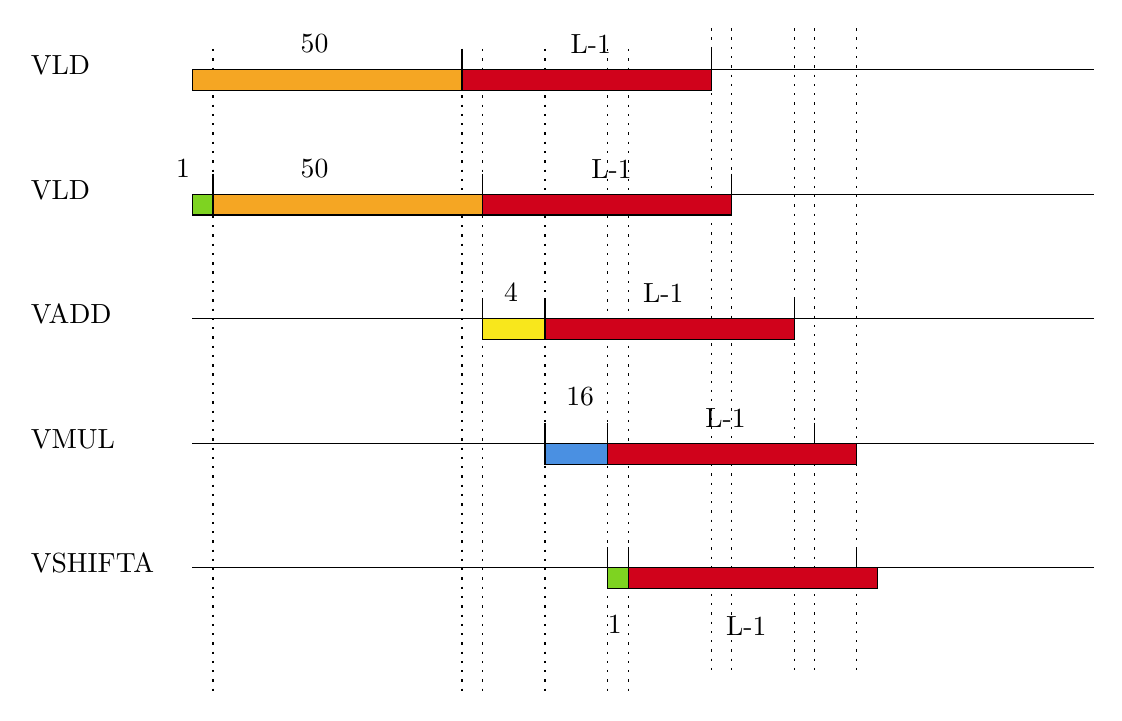
\begin{tikzpicture}[x=0.75pt,y=0.75pt,yscale=-1,xscale=1]
		%uncomment if require: \path (0,443); %set diagram left start at 0, and has height of 443
		
		%Straight Lines [id:da4056751599361361] 
		\draw    (110,120) -- (544.33,120) ;
		%Straight Lines [id:da7857853563029675] 
		\draw    (110,60) -- (544.33,60) ;
		%Straight Lines [id:da0005831337046342533] 
		\draw    (110,240) -- (544.33,240) ;
		%Straight Lines [id:da08536951785383828] 
		\draw    (110,180) -- (544.33,180) ;
		%Straight Lines [id:da6201197043178086] 
		\draw    (110,300) -- (544.33,300) ;
		%Straight Lines [id:da3381599644550526] 
		\draw    (120,110) -- (120,130) ;
		%Straight Lines [id:da6690442976711715] 
		\draw    (240,50) -- (240,70) ;
		%Straight Lines [id:da4406342150002809] 
		\draw    (360,50) -- (360,70) ;
		%Straight Lines [id:da5043168469308337] 
		\draw    (250,110) -- (250,130) ;
		%Straight Lines [id:da4666662992364088] 
		\draw    (250,170) -- (250,190) ;
		%Straight Lines [id:da5939922983419239] 
		\draw    (280,170) -- (280,190) ;
		%Straight Lines [id:da5189530821446637] 
		\draw    (280,230) -- (280,250) ;
		%Straight Lines [id:da3663031714665561] 
		\draw    (310,230) -- (310,250) ;
		%Straight Lines [id:da9338209659786427] 
		\draw    (310,290) -- (310,310) ;
		%Straight Lines [id:da18523939863568195] 
		\draw    (320,290) -- (320,310) ;
		%Straight Lines [id:da4724321762569552] 
		\draw    (430,290) -- (430,310) ;
		%Straight Lines [id:da6693610828912262] 
		\draw    (370,110) -- (370,130) ;
		%Straight Lines [id:da6270296838242602] 
		\draw    (400,170) -- (400,190) ;
		%Straight Lines [id:da3364447390724097] 
		\draw    (410,230) -- (410,250) ;
		%Straight Lines [id:da18370753336787038] 
		\draw  [dash pattern={on 0.84pt off 2.51pt}]  (240,50) -- (240,360) ;
		%Straight Lines [id:da7376921896027557] 
		\draw  [dash pattern={on 0.84pt off 2.51pt}]  (120,50) -- (120,360) ;
		%Straight Lines [id:da15315329332541538] 
		\draw  [dash pattern={on 0.84pt off 2.51pt}]  (250,50) -- (250,360) ;
		%Straight Lines [id:da37589207976578365] 
		\draw  [dash pattern={on 0.84pt off 2.51pt}]  (320,50) -- (320,360) ;
		%Straight Lines [id:da041269737704872744] 
		\draw  [dash pattern={on 0.84pt off 2.51pt}]  (310,50) -- (310,360) ;
		%Straight Lines [id:da0925947929511568] 
		\draw  [dash pattern={on 0.84pt off 2.51pt}]  (280,50) -- (280,360) ;
		%Straight Lines [id:da5616542319228255] 
		\draw  [dash pattern={on 0.84pt off 2.51pt}]  (360,40) -- (360,350) ;
		%Straight Lines [id:da42573647296341766] 
		\draw  [dash pattern={on 0.84pt off 2.51pt}]  (370,40) -- (370,350) ;
		%Straight Lines [id:da6610979565268893] 
		\draw  [dash pattern={on 0.84pt off 2.51pt}]  (400,40) -- (400,350) ;
		%Straight Lines [id:da7859095956814592] 
		\draw  [dash pattern={on 0.84pt off 2.51pt}]  (430,40) -- (430,350) ;
		%Straight Lines [id:da257640124640119] 
		\draw  [dash pattern={on 0.84pt off 2.51pt}]  (410,40) -- (410,350) ;
		%Shape: Rectangle [id:dp4429906273938109] 
		\draw  [fill={rgb, 255:red, 245; green, 166; blue, 35 }  ,fill opacity=1 ] (120,120) -- (250,120) -- (250,130) -- (120,130) -- cycle ;
		%Shape: Rectangle [id:dp1822788157156785] 
		\draw  [fill={rgb, 255:red, 245; green, 166; blue, 35 }  ,fill opacity=1 ] (110,60) -- (240,60) -- (240,70) -- (110,70) -- cycle ;
		%Shape: Rectangle [id:dp08196264729456515] 
		\draw  [fill={rgb, 255:red, 126; green, 211; blue, 33 }  ,fill opacity=1 ] (110,120) -- (120,120) -- (120,130) -- (110,130) -- cycle ;
		%Shape: Rectangle [id:dp5451042586209953] 
		\draw  [fill={rgb, 255:red, 208; green, 2; blue, 27 }  ,fill opacity=1 ] (240,60) -- (360,60) -- (360,70) -- (240,70) -- cycle ;
		%Shape: Rectangle [id:dp011752207493361144] 
		\draw  [fill={rgb, 255:red, 208; green, 2; blue, 27 }  ,fill opacity=1 ] (250,120) -- (370,120) -- (370,130) -- (250,130) -- cycle ;
		%Shape: Rectangle [id:dp8185125888655953] 
		\draw  [fill={rgb, 255:red, 248; green, 231; blue, 28 }  ,fill opacity=1 ] (250,180) -- (280,180) -- (280,190) -- (250,190) -- cycle ;
		%Shape: Rectangle [id:dp9099220139820643] 
		\draw  [fill={rgb, 255:red, 208; green, 2; blue, 27 }  ,fill opacity=1 ] (280,180) -- (400,180) -- (400,190) -- (280,190) -- cycle ;
		%Shape: Rectangle [id:dp3189647281403514] 
		\draw  [fill={rgb, 255:red, 208; green, 2; blue, 27 }  ,fill opacity=1 ] (310,240) -- (430,240) -- (430,250) -- (310,250) -- cycle ;
		%Shape: Rectangle [id:dp7815445165305275] 
		\draw  [fill={rgb, 255:red, 208; green, 2; blue, 27 }  ,fill opacity=1 ] (320,300) -- (440,300) -- (440,310) -- (320,310) -- cycle ;
		%Shape: Rectangle [id:dp8750624797959485] 
		\draw  [fill={rgb, 255:red, 74; green, 144; blue, 226 }  ,fill opacity=1 ] (280,240) -- (310,240) -- (310,250) -- (280,250) -- cycle ;
		%Shape: Rectangle [id:dp8876681326661466] 
		\draw  [fill={rgb, 255:red, 126; green, 211; blue, 33 }  ,fill opacity=1 ] (310,300) -- (320,300) -- (320,310) -- (310,310) -- cycle ;
		
		% Text Node
		\draw (161,42) node [anchor=north west][inner sep=0.75pt]   [align=left] {50};
		% Text Node
		\draw (291,42) node [anchor=north west][inner sep=0.75pt]   [align=left] {L-1};
		% Text Node
		\draw (101,102) node [anchor=north west][inner sep=0.75pt]   [align=left] {1};
		% Text Node
		\draw (161,102) node [anchor=north west][inner sep=0.75pt]   [align=left] {50};
		% Text Node
		\draw (301,102) node [anchor=north west][inner sep=0.75pt]   [align=left] {L-1};
		% Text Node
		\draw (326,162) node [anchor=north west][inner sep=0.75pt]   [align=left] {L-1};
		% Text Node
		\draw (259,162) node [anchor=north west][inner sep=0.75pt]   [align=left] {4};
		% Text Node
		\draw (289,212) node [anchor=north west][inner sep=0.75pt]   [align=left] {16};
		% Text Node
		\draw (356,222) node [anchor=north west][inner sep=0.75pt]   [align=left] {L-1};
		% Text Node
		\draw (309,322) node [anchor=north west][inner sep=0.75pt]   [align=left] {1};
		% Text Node
		\draw (366,322) node [anchor=north west][inner sep=0.75pt]   [align=left] {L-1};
		% Text Node
		\draw (31,52) node [anchor=north west][inner sep=0.75pt]   [align=left] {VLD};
		% Text Node
		\draw (31,112) node [anchor=north west][inner sep=0.75pt]   [align=left] {VLD};
		% Text Node
		\draw (31,172) node [anchor=north west][inner sep=0.75pt]   [align=left] {VADD};
		% Text Node
		\draw (31,232) node [anchor=north west][inner sep=0.75pt]   [align=left] {VMUL};
		% Text Node
		\draw (31,292) node [anchor=north west][inner sep=0.75pt]   [align=left] {VSHIFTA};
		
		
	\end{tikzpicture}
	
	\newpage

	
	
	According to the picture below:
	
	$$1 + 50 + L-1 + 4 + L-1 + 16 + L-1 + 1 + L-1 = 228 ~~\text{cycles}$$
	
	
	
	


\tikzset{every picture/.style={line width=0.75pt}} %set default line width to 0.75pt        

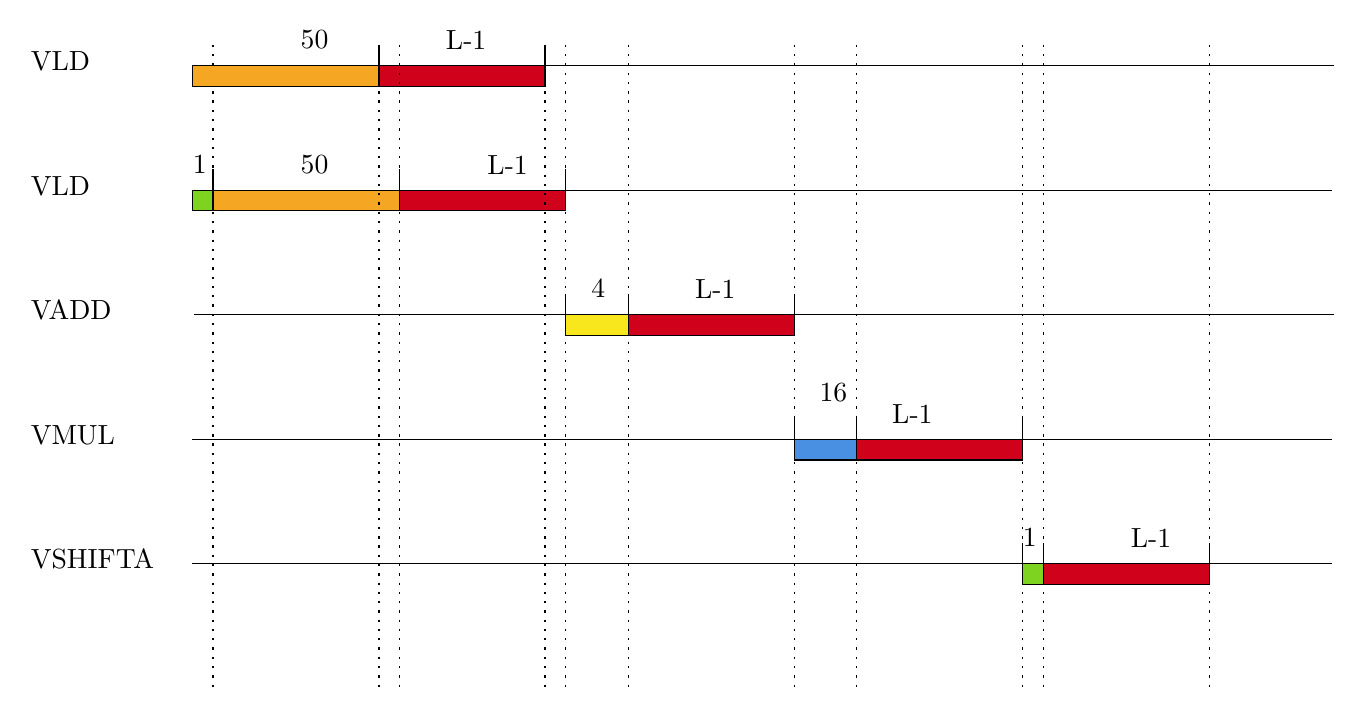
\begin{tikzpicture}[x=0.75pt,y=0.75pt,yscale=-1,xscale=1]
	%uncomment if require: \path (0,443); %set diagram left start at 0, and has height of 443
	
	%Straight Lines [id:da4056751599361361] 
	\draw    (110,120) -- (659.16,120) ;
	%Straight Lines [id:da7857853563029675] 
	\draw    (110.84,60) -- (660,60) ;
	%Straight Lines [id:da0005831337046342533] 
	\draw    (110,240) -- (659.16,240) ;
	%Straight Lines [id:da08536951785383828] 
	\draw    (110.84,180) -- (660,180) ;
	%Straight Lines [id:da6201197043178086] 
	\draw    (110,300) -- (659.16,300) ;
	%Straight Lines [id:da3381599644550526] 
	\draw    (120,110) -- (120,130) ;
	%Straight Lines [id:da6690442976711715] 
	\draw    (200,50) -- (200,70) ;
	%Straight Lines [id:da4406342150002809] 
	\draw    (280,50) -- (280,70) ;
	%Straight Lines [id:da5043168469308337] 
	\draw    (210,110) -- (210,130) ;
	%Straight Lines [id:da4666662992364088] 
	\draw    (320,170) -- (320,190) ;
	%Straight Lines [id:da5939922983419239] 
	\draw    (290,170) -- (290,190) ;
	%Straight Lines [id:da5189530821446637] 
	\draw    (400,230) -- (400,250) ;
	%Straight Lines [id:da3663031714665561] 
	\draw    (510,230) -- (510,250) ;
	%Straight Lines [id:da9338209659786427] 
	\draw    (510,290) -- (510,310) ;
	%Straight Lines [id:da18523939863568195] 
	\draw    (600,290) -- (600,310) ;
	%Straight Lines [id:da4724321762569552] 
	\draw    (520,290) -- (520,310) ;
	%Straight Lines [id:da6693610828912262] 
	\draw    (290,110) -- (290,130) ;
	%Straight Lines [id:da6270296838242602] 
	\draw    (400,170) -- (400,190) ;
	%Straight Lines [id:da3364447390724097] 
	\draw    (430,230) -- (430,250) ;
	%Straight Lines [id:da7376921896027557] 
	\draw  [dash pattern={on 0.84pt off 2.51pt}]  (120,50) -- (120,360) ;
	%Shape: Rectangle [id:dp4429906273938109] 
	\draw  [fill={rgb, 255:red, 245; green, 166; blue, 35 }  ,fill opacity=1 ] (120,120) -- (210,120) -- (210,130) -- (120,130) -- cycle ;
	%Shape: Rectangle [id:dp1822788157156785] 
	\draw  [fill={rgb, 255:red, 245; green, 166; blue, 35 }  ,fill opacity=1 ] (110,60) -- (200,60) -- (200,70) -- (110,70) -- cycle ;
	%Shape: Rectangle [id:dp08196264729456515] 
	\draw  [fill={rgb, 255:red, 126; green, 211; blue, 33 }  ,fill opacity=1 ] (110,120) -- (120,120) -- (120,130) -- (110,130) -- cycle ;
	%Shape: Rectangle [id:dp5451042586209953] 
	\draw  [fill={rgb, 255:red, 208; green, 2; blue, 27 }  ,fill opacity=1 ] (200,60) -- (280,60) -- (280,70) -- (200,70) -- cycle ;
	%Shape: Rectangle [id:dp8185125888655953] 
	\draw  [fill={rgb, 255:red, 248; green, 231; blue, 28 }  ,fill opacity=1 ] (290,180) -- (320,180) -- (320,190) -- (290,190) -- cycle ;
	%Shape: Rectangle [id:dp8750624797959485] 
	\draw  [fill={rgb, 255:red, 74; green, 144; blue, 226 }  ,fill opacity=1 ] (400,240) -- (430,240) -- (430,250) -- (400,250) -- cycle ;
	%Shape: Rectangle [id:dp8876681326661466] 
	\draw  [fill={rgb, 255:red, 126; green, 211; blue, 33 }  ,fill opacity=1 ] (510,300) -- (520,300) -- (520,310) -- (510,310) -- cycle ;
	%Shape: Rectangle [id:dp5222870449478838] 
	\draw  [fill={rgb, 255:red, 208; green, 2; blue, 27 }  ,fill opacity=1 ] (210,120) -- (290,120) -- (290,130) -- (210,130) -- cycle ;
	%Shape: Rectangle [id:dp39467189134125924] 
	\draw  [fill={rgb, 255:red, 208; green, 2; blue, 27 }  ,fill opacity=1 ] (320,180) -- (400,180) -- (400,190) -- (320,190) -- cycle ;
	%Shape: Rectangle [id:dp0884298735116551] 
	\draw  [fill={rgb, 255:red, 208; green, 2; blue, 27 }  ,fill opacity=1 ] (430,240) -- (510,240) -- (510,250) -- (430,250) -- cycle ;
	%Shape: Rectangle [id:dp3654545762165393] 
	\draw  [fill={rgb, 255:red, 208; green, 2; blue, 27 }  ,fill opacity=1 ] (520,300) -- (600,300) -- (600,310) -- (520,310) -- cycle ;
	%Straight Lines [id:da42028134468685097] 
	\draw  [dash pattern={on 0.84pt off 2.51pt}]  (200,50) -- (200,360) ;
	%Straight Lines [id:da8915315648394992] 
	\draw  [dash pattern={on 0.84pt off 2.51pt}]  (210,50) -- (210,360) ;
	%Straight Lines [id:da7918867335054993] 
	\draw  [dash pattern={on 0.84pt off 2.51pt}]  (280,50) -- (280,360) ;
	%Straight Lines [id:da33968785689214775] 
	\draw  [dash pattern={on 0.84pt off 2.51pt}]  (290,50) -- (290,360) ;
	%Straight Lines [id:da5555941612701312] 
	\draw  [dash pattern={on 0.84pt off 2.51pt}]  (320,50) -- (320,360) ;
	%Straight Lines [id:da044833338423639235] 
	\draw  [dash pattern={on 0.84pt off 2.51pt}]  (400,50) -- (400,360) ;
	%Straight Lines [id:da6892931550715751] 
	\draw  [dash pattern={on 0.84pt off 2.51pt}]  (430,50) -- (430,360) ;
	%Straight Lines [id:da6999989598549299] 
	\draw  [dash pattern={on 0.84pt off 2.51pt}]  (510,50) -- (510,360) ;
	%Straight Lines [id:da2711377582239678] 
	\draw  [dash pattern={on 0.84pt off 2.51pt}]  (520,50) -- (520,360) ;
	%Straight Lines [id:da23727116063665887] 
	\draw  [dash pattern={on 0.84pt off 2.51pt}]  (600,50) -- (600,360) ;
	
	% Text Node
	\draw (161,42) node [anchor=north west][inner sep=0.75pt]   [align=left] {50};
	% Text Node
	\draw (231,42) node [anchor=north west][inner sep=0.75pt]   [align=left] {L-1};
	% Text Node
	\draw (109,102) node [anchor=north west][inner sep=0.75pt]   [align=left] {1};
	% Text Node
	\draw (161,102) node [anchor=north west][inner sep=0.75pt]   [align=left] {50};
	% Text Node
	\draw (251,102) node [anchor=north west][inner sep=0.75pt]   [align=left] {L-1};
	% Text Node
	\draw (351,162) node [anchor=north west][inner sep=0.75pt]   [align=left] {L-1};
	% Text Node
	\draw (301,162) node [anchor=north west][inner sep=0.75pt]   [align=left] {4};
	% Text Node
	\draw (411,212) node [anchor=north west][inner sep=0.75pt]   [align=left] {16};
	% Text Node
	\draw (446,222) node [anchor=north west][inner sep=0.75pt]   [align=left] {L-1};
	% Text Node
	\draw (31,52) node [anchor=north west][inner sep=0.75pt]   [align=left] {VLD};
	% Text Node
	\draw (31,112) node [anchor=north west][inner sep=0.75pt]   [align=left] {VLD};
	% Text Node
	\draw (31,172) node [anchor=north west][inner sep=0.75pt]   [align=left] {VADD};
	% Text Node
	\draw (31,232) node [anchor=north west][inner sep=0.75pt]   [align=left] {VMUL};
	% Text Node
	\draw (31,292) node [anchor=north west][inner sep=0.75pt]   [align=left] {VSHIFTA};
	% Text Node
	\draw (561,282) node [anchor=north west][inner sep=0.75pt]   [align=left] {L-1};
	% Text Node
	\draw (509,282) node [anchor=north west][inner sep=0.75pt]   [align=left] {1};
	
	
\end{tikzpicture}
\newpage

\item 
In this case there will actually be two stages of load. The bank size will be $32$ and we want to get values till $40$. Therefore based on the picture below, the answer will be:

$$1+50+50+7+4+16+1 = 129 ~~ \text{cycles}$$



\tikzset{every picture/.style={line width=0.75pt}} %set default line width to 0.75pt        

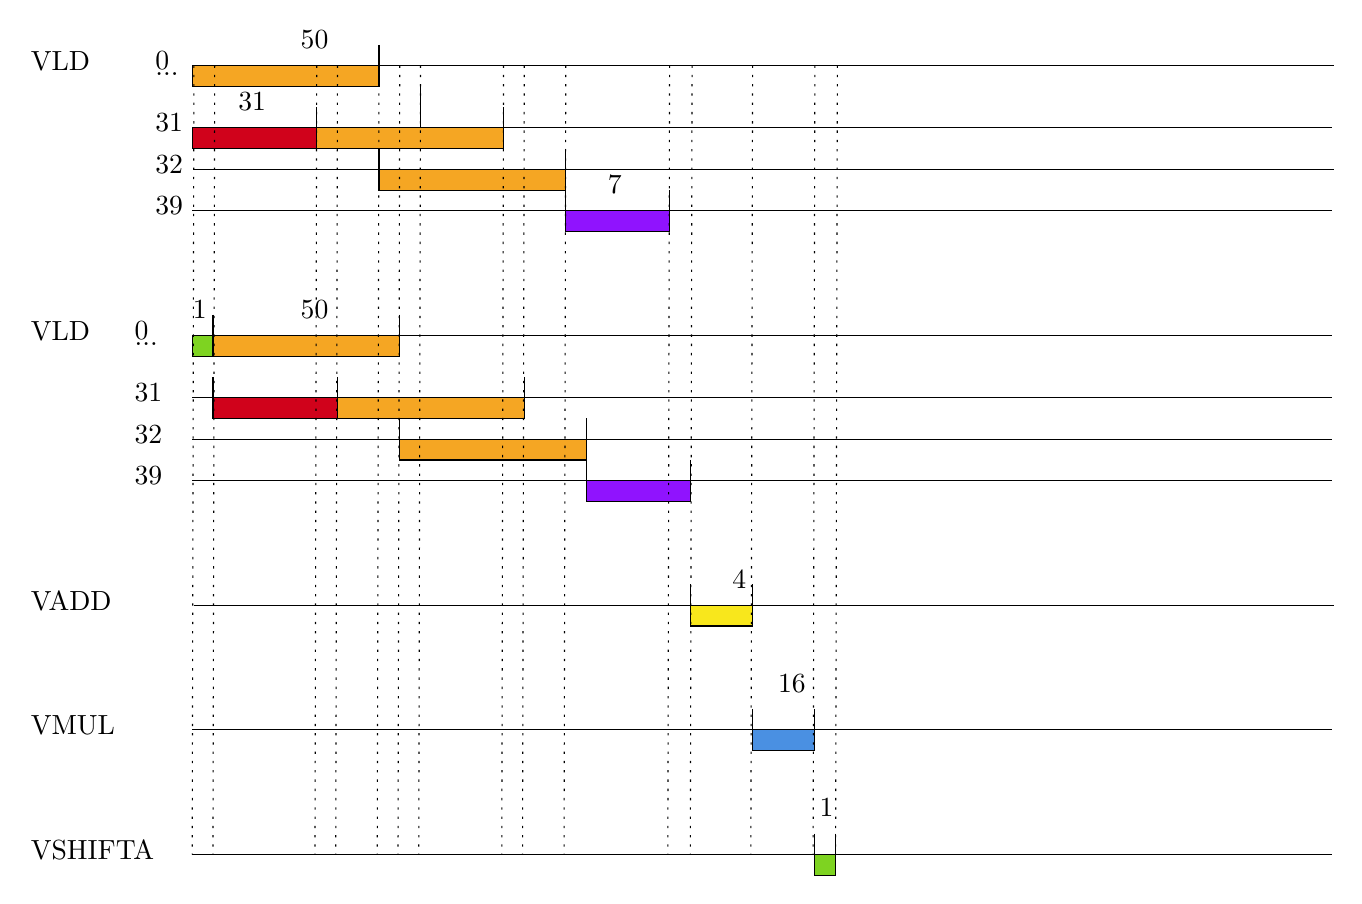
\begin{tikzpicture}[x=0.75pt,y=0.75pt,yscale=-1,xscale=1]
	%uncomment if require: \path (0,477); %set diagram left start at 0, and has height of 477
	
	%Straight Lines [id:da4056751599361361] 
	\draw    (110,190) -- (659.16,190) ;
	%Straight Lines [id:da7857853563029675] 
	\draw    (110.84,60) -- (660,60) ;
	%Straight Lines [id:da0005831337046342533] 
	\draw    (110,380) -- (659.16,380) ;
	%Straight Lines [id:da08536951785383828] 
	\draw    (110.84,320) -- (660,320) ;
	%Straight Lines [id:da6201197043178086] 
	\draw    (110,440) -- (659.16,440) ;
	%Straight Lines [id:da3381599644550526] 
	\draw    (120,180) -- (120,200) ;
	%Straight Lines [id:da6690442976711715] 
	\draw    (200,50) -- (200,70) ;
	%Straight Lines [id:da5043168469308337] 
	\draw    (210,180) -- (210,200) ;
	%Straight Lines [id:da4666662992364088] 
	\draw    (380,310) -- (380,330) ;
	%Straight Lines [id:da5939922983419239] 
	\draw    (350,310) -- (350,330) ;
	%Straight Lines [id:da5189530821446637] 
	\draw    (380,370) -- (380,390) ;
	%Straight Lines [id:da3663031714665561] 
	\draw    (410,430) -- (410,450) ;
	%Straight Lines [id:da6693610828912262] 
	\draw    (210,230) -- (210,250) ;
	%Straight Lines [id:da6270296838242602] 
	\draw    (420,430) -- (420,450) ;
	%Straight Lines [id:da3364447390724097] 
	\draw    (410,370) -- (410,390) ;
	%Shape: Rectangle [id:dp4429906273938109] 
	\draw  [fill={rgb, 255:red, 245; green, 166; blue, 35 }  ,fill opacity=1 ] (120,190) -- (210,190) -- (210,200) -- (120,200) -- cycle ;
	%Shape: Rectangle [id:dp1822788157156785] 
	\draw  [fill={rgb, 255:red, 245; green, 166; blue, 35 }  ,fill opacity=1 ] (110,60) -- (200,60) -- (200,70) -- (110,70) -- cycle ;
	%Shape: Rectangle [id:dp08196264729456515] 
	\draw  [fill={rgb, 255:red, 126; green, 211; blue, 33 }  ,fill opacity=1 ] (110,190) -- (120,190) -- (120,200) -- (110,200) -- cycle ;
	%Shape: Rectangle [id:dp8185125888655953] 
	\draw  [fill={rgb, 255:red, 248; green, 231; blue, 28 }  ,fill opacity=1 ] (350,320) -- (380,320) -- (380,330) -- (350,330) -- cycle ;
	%Shape: Rectangle [id:dp8750624797959485] 
	\draw  [fill={rgb, 255:red, 74; green, 144; blue, 226 }  ,fill opacity=1 ] (380,380) -- (410,380) -- (410,390) -- (380,390) -- cycle ;
	%Shape: Rectangle [id:dp8876681326661466] 
	\draw  [fill={rgb, 255:red, 126; green, 211; blue, 33 }  ,fill opacity=1 ] (410,440) -- (420,440) -- (420,450) -- (410,450) -- cycle ;
	%Straight Lines [id:da23727116063665887] 
	\draw  [dash pattern={on 0.84pt off 2.51pt}]  (110.84,60) -- (110,440) ;
	%Straight Lines [id:da08122823956380754] 
	\draw    (110,90) -- (659.16,90) ;
	%Straight Lines [id:da7973830028082882] 
	\draw    (110.84,110) -- (660,110) ;
	%Straight Lines [id:da7451371464749763] 
	\draw    (110,130) -- (659.16,130) ;
	%Straight Lines [id:da10790214759688688] 
	\draw    (110,220) -- (659.16,220) ;
	%Straight Lines [id:da4336914484638976] 
	\draw    (110,240) -- (659.16,240) ;
	%Straight Lines [id:da3470047883941272] 
	\draw    (110,260) -- (659.16,260) ;
	%Shape: Rectangle [id:dp6208090158033317] 
	\draw  [fill={rgb, 255:red, 208; green, 2; blue, 27 }  ,fill opacity=1 ] (110,90) -- (170,90) -- (170,100) -- (110,100) -- cycle ;
	%Straight Lines [id:da038551515414996906] 
	\draw    (170,80) -- (170,100) ;
	%Shape: Rectangle [id:dp42009030750924836] 
	\draw  [fill={rgb, 255:red, 245; green, 166; blue, 35 }  ,fill opacity=1 ] (170,90) -- (260,90) -- (260,100) -- (170,100) -- cycle ;
	%Shape: Rectangle [id:dp9723299541875654] 
	\draw  [fill={rgb, 255:red, 245; green, 166; blue, 35 }  ,fill opacity=1 ] (200,110) -- (290,110) -- (290,120) -- (200,120) -- cycle ;
	%Shape: Rectangle [id:dp06086095348752241] 
	\draw  [fill={rgb, 255:red, 144; green, 19; blue, 254 }  ,fill opacity=1 ] (290,130) -- (340,130) -- (340,140) -- (290,140) -- cycle ;
	%Shape: Rectangle [id:dp12373272769147081] 
	\draw  [fill={rgb, 255:red, 208; green, 2; blue, 27 }  ,fill opacity=1 ] (120,220) -- (180,220) -- (180,230) -- (120,230) -- cycle ;
	%Shape: Rectangle [id:dp5110066537877145] 
	\draw  [fill={rgb, 255:red, 245; green, 166; blue, 35 }  ,fill opacity=1 ] (180,220) -- (270,220) -- (270,230) -- (180,230) -- cycle ;
	%Shape: Rectangle [id:dp5509382448186515] 
	\draw  [fill={rgb, 255:red, 245; green, 166; blue, 35 }  ,fill opacity=1 ] (210,240) -- (300,240) -- (300,250) -- (210,250) -- cycle ;
	%Shape: Rectangle [id:dp7786777532162477] 
	\draw  [fill={rgb, 255:red, 144; green, 19; blue, 254 }  ,fill opacity=1 ] (300,260) -- (350,260) -- (350,270) -- (300,270) -- cycle ;
	%Straight Lines [id:da9764275045432966] 
	\draw    (260,80) -- (260,100) ;
	%Straight Lines [id:da9651093378150155] 
	\draw    (200,100) -- (200,120) ;
	%Straight Lines [id:da6816459573340143] 
	\draw    (290,100) -- (290,120) ;
	%Straight Lines [id:da2805486235281178] 
	\draw    (290,120) -- (290,140) ;
	%Straight Lines [id:da34238862980875817] 
	\draw    (340,120) -- (340,140) ;
	%Straight Lines [id:da44919757358810686] 
	\draw    (120,210) -- (120,230) ;
	%Straight Lines [id:da3237240924376801] 
	\draw    (180,210) -- (180,230) ;
	%Straight Lines [id:da4060680071317282] 
	\draw    (270,210) -- (270,230) ;
	%Straight Lines [id:da6915775353087534] 
	\draw    (300,230) -- (300,250) ;
	%Straight Lines [id:da2619128724658568] 
	\draw    (300,250) -- (300,270) ;
	%Straight Lines [id:da7533101316913591] 
	\draw    (350,250) -- (350,270) ;
	%Straight Lines [id:da26275266184661716] 
	\draw    (220,70) -- (220,90) ;
	%Straight Lines [id:da41421192180653943] 
	\draw    (220,70) -- (220,90) ;
	%Straight Lines [id:da7248839973591787] 
	\draw  [dash pattern={on 0.84pt off 2.51pt}]  (120.84,60) -- (120,440) ;
	%Straight Lines [id:da9053990239408511] 
	\draw  [dash pattern={on 0.84pt off 2.51pt}]  (170,60) -- (169.16,440) ;
	%Straight Lines [id:da45358129593940233] 
	\draw  [dash pattern={on 0.84pt off 2.51pt}]  (180,60) -- (179.16,440) ;
	%Straight Lines [id:da30499088385818207] 
	\draw  [dash pattern={on 0.84pt off 2.51pt}]  (200,60) -- (199.16,440) ;
	%Straight Lines [id:da9266516875315556] 
	\draw  [dash pattern={on 0.84pt off 2.51pt}]  (210,60) -- (209.16,440) ;
	%Straight Lines [id:da29722141363981147] 
	\draw  [dash pattern={on 0.84pt off 2.51pt}]  (220,60) -- (219.16,440) ;
	%Straight Lines [id:da3137655732839948] 
	\draw  [dash pattern={on 0.84pt off 2.51pt}]  (260,60) -- (259.16,440) ;
	%Straight Lines [id:da4482293757768472] 
	\draw  [dash pattern={on 0.84pt off 2.51pt}]  (270,60) -- (269.16,440) ;
	%Straight Lines [id:da7899419768138523] 
	\draw  [dash pattern={on 0.84pt off 2.51pt}]  (290,60) -- (289.16,440) ;
	%Straight Lines [id:da5700616580091868] 
	\draw  [dash pattern={on 0.84pt off 2.51pt}]  (340,60) -- (339.16,440) ;
	%Straight Lines [id:da5560792390077038] 
	\draw  [dash pattern={on 0.84pt off 2.51pt}]  (350.84,60) -- (350,440) ;
	%Straight Lines [id:da8108178784855287] 
	\draw  [dash pattern={on 0.84pt off 2.51pt}]  (380,60) -- (379.16,440) ;
	%Straight Lines [id:da2857372509935756] 
	\draw  [dash pattern={on 0.84pt off 2.51pt}]  (410,60) -- (409.16,440) ;
	%Straight Lines [id:da631553380866289] 
	\draw  [dash pattern={on 0.84pt off 2.51pt}]  (420.84,60) -- (420,440) ;
	
	% Text Node
	\draw (161,42) node [anchor=north west][inner sep=0.75pt]   [align=left] {50};
	% Text Node
	\draw (109,172) node [anchor=north west][inner sep=0.75pt]   [align=left] {1};
	% Text Node
	\draw (161,172) node [anchor=north west][inner sep=0.75pt]   [align=left] {50};
	% Text Node
	\draw (369,302) node [anchor=north west][inner sep=0.75pt]   [align=left] {4};
	% Text Node
	\draw (391,352) node [anchor=north west][inner sep=0.75pt]   [align=left] {16};
	% Text Node
	\draw (31,52) node [anchor=north west][inner sep=0.75pt]   [align=left] {VLD};
	% Text Node
	\draw (31,182) node [anchor=north west][inner sep=0.75pt]   [align=left] {VLD};
	% Text Node
	\draw (31,312) node [anchor=north west][inner sep=0.75pt]   [align=left] {VADD};
	% Text Node
	\draw (31,372) node [anchor=north west][inner sep=0.75pt]   [align=left] {VMUL};
	% Text Node
	\draw (31,432) node [anchor=north west][inner sep=0.75pt]   [align=left] {VSHIFTA};
	% Text Node
	\draw (91,52) node [anchor=north west][inner sep=0.75pt]   [align=left] {0};
	% Text Node
	\draw (91,62) node [anchor=north west][inner sep=0.75pt]   [align=left] {...};
	% Text Node
	\draw (91,82) node [anchor=north west][inner sep=0.75pt]   [align=left] {31};
	% Text Node
	\draw (91,102) node [anchor=north west][inner sep=0.75pt]   [align=left] {32};
	% Text Node
	\draw (91,122) node [anchor=north west][inner sep=0.75pt]   [align=left] {39};
	% Text Node
	\draw (81,182) node [anchor=north west][inner sep=0.75pt]   [align=left] {0};
	% Text Node
	\draw (81,192) node [anchor=north west][inner sep=0.75pt]   [align=left] {...};
	% Text Node
	\draw (81,212) node [anchor=north west][inner sep=0.75pt]   [align=left] {31};
	% Text Node
	\draw (81,232) node [anchor=north west][inner sep=0.75pt]   [align=left] {32};
	% Text Node
	\draw (81,252) node [anchor=north west][inner sep=0.75pt]   [align=left] {39};
	% Text Node
	\draw (411,412) node [anchor=north west][inner sep=0.75pt]   [align=left] {1};
	% Text Node
	\draw (131,72) node [anchor=north west][inner sep=0.75pt]   [align=left] {31};
	% Text Node
	\draw (309,112) node [anchor=north west][inner sep=0.75pt]   [align=left] {7};
	
	
\end{tikzpicture}

	
By the pattern found until now, we can say:

$$x \times 50 + 1 +7 +4 + 16 + 1 = 279 \Rightarrow  x= 5$$

The following power of two to $5$ is $8$. So the answer is $8$ banks.

\item 

Row-Buffer Conflict causes it. It means the interleaving of vector accesses of cores on the shared memory. For example, core 0 wants to access a vector that is mapped to bank 0, and at the same time, independent of core 0, core 0 also wants to access another vector that is mapped to bank 0. As the memory is shared, this will cause a Row-Buffer conflict.


To solve the problem, the architect could partition the memory mapping or use advanced memory scheduling techniques that reorder memory access to minimize conflicts.

Partitioning the memory mapping can be done in many ways. One of them is to assign colors to each partition and only allow access to the partition for processes (threads) that are associated with that specific color \cite{AhrenInvestigatingDB}.
\end{enumerate}


\nocite{*}

\bibliographystyle{plain}
\bibliography{refs}

\newpage

\section{Question Four}
\begin{enumerate}[label=\alph*.]
	
	\item 
	Array Processor. An array processor will require 16 functional units that can do all different operations because they all need to do the same operation simultaneously. But the vector processor needs only one because it should do different jobs simultaneously, and each part of this functional unit can do the job assigned to them at the same time.
	
	\item 
	
	$$5 + (L-1) + 5 + (L-1) + 15 + (L-1) = 52 \Rightarrow$$ 
	
	$$VLEN = L = 10$$
	
	On an array processor, it will take $5+5+15=25$ cycles. There are data dependencies between operations, and one should end before the other one can begin.
	
	\item 
	$$20 + 20 + (L -1)  + 5 + (L-1) + 1 + (L-1) + 20 + (L-1) = 94 \Rightarrow$$
	$$VLEN = L = 8$$
	
	The two first Loads can actually be done in parallel. Therefore we will only have $L-1$ for them. The $L-1$ of the first one is actually interleaved in the second one.
	
	
	
	\item 
	
	
	We assume the number of banks is a power of two.
	
	$$20 \times (\frac{16}{b}) + 20 \times (\frac{16}{b}) + (b-1) + 5 + (L-1) + 1 + (L-1) + 20 \times (\frac{16}{b}) + (b-1) = 170 \rightarrow$$
	
	$$b=8$$
	
	
	The $b-1$ part is actually because if, for example, we have $8$ banks and data is of $VLEN = 16$, then at the first eight cycles, we can initiate loads of 8 of the data and then we must wait until the first one ends to initiate the next part. In this case, if we start at cycle 0, the whole load will end at $20 + 20 + 7=47$.
	
	
\end{enumerate}


\newpage




\end{document}



